% !TEX root = ../../main.tex
\section{Data Sets}\label{sec:data_sets}
In the previous chapter we have applied our method \gls{ocs-hats} to the artificial data sets from Camci~\cite{camci2010change} and Takeuchi and Yamanishi~\cite{takeuchi2006unifying}.
In this chapter we apply the method to real-world data sets.
The data sets come from inertial sensor data recorded during human activities, such as walking, running, ascending and descending stairs, and standing still.
To compare our results with other research, we have tried to apply \gls{ocs-hats} to two commonly used data sets.
The first is the data from the \gls{wisdm} lab \cite{kwapisz2011activity}.
As an excerpt from the data in \Cref{fig:wisdm_excerpt} shows, the activities are recorded non-continuous.
Whilst this data set is convenient for activity classification, it does not allow for detection of change points.
Even if the gap between the activities would be removed, the transition segments between activities would still be missing and thus the data set would not reflect continuous recordings.
The other commonly used data set is the \gls{uci-har} from the Machine Learning Repository and originates from \cite{anguita2012human}.
As shown in an except in \Cref{fig:uci_annotated}, the labeling to the data segments seems to be incorrect.
Furthermore, it is not clear how the data is recorded and whether all activities are performed continuously.

\begin{figure}
\centering
  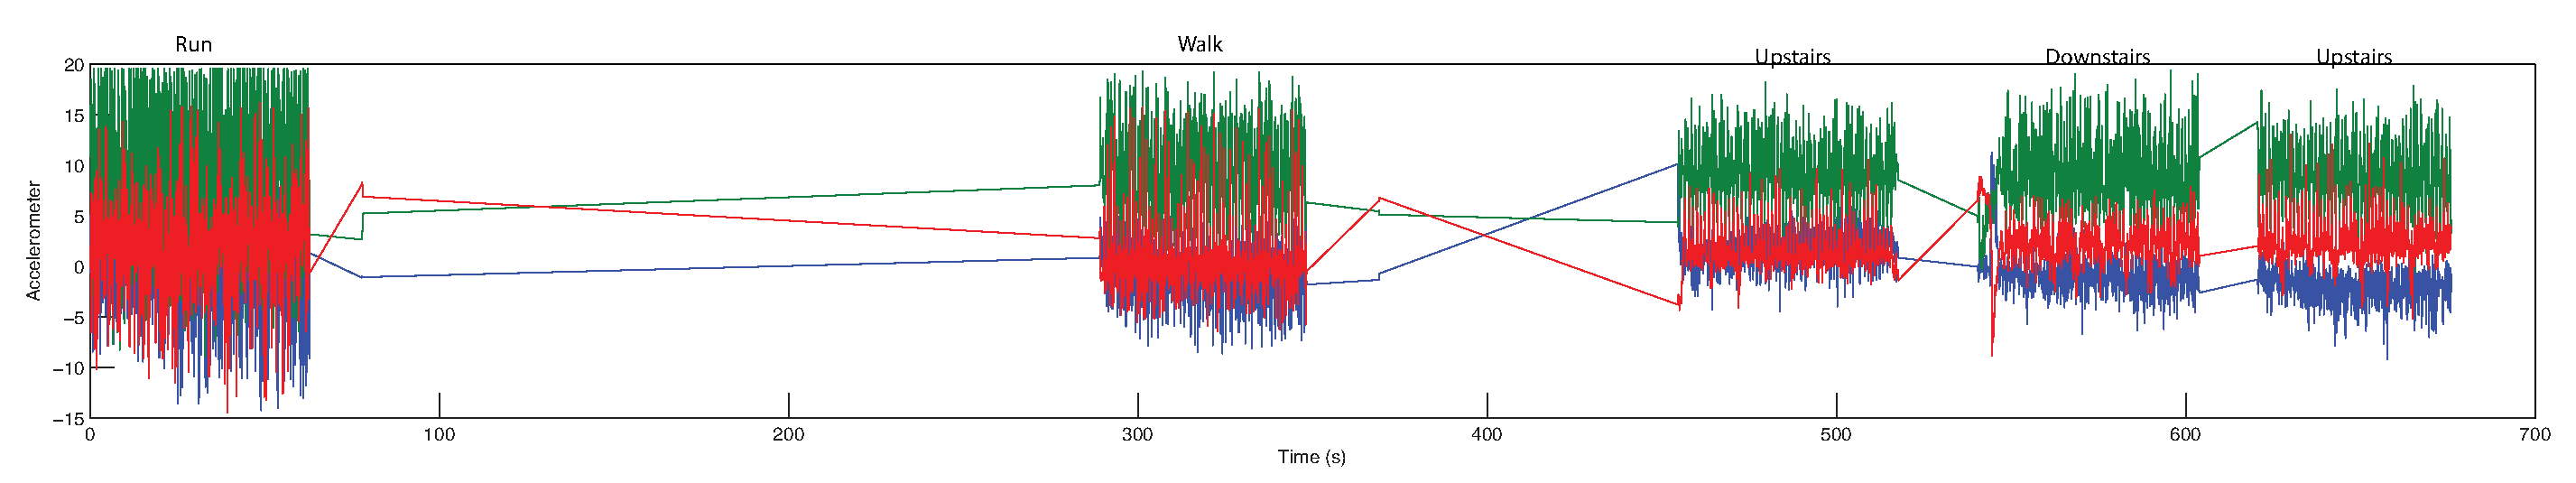
\includegraphics[width=1\textwidth]{./Figures/Chapter6/data_collection/wisdm_excerpt.eps}
  \caption[WISDM Excerpt]{Excerpt from the WISDM data set \cite{kwapisz2011activity}. First five activities for subject $33$ are displayed. Due to the discontinuous nature of the recordings, this data set can not be used for change detection.}
  \label{fig:wisdm_excerpt}
\end{figure}

\begin{figure}
\centering
  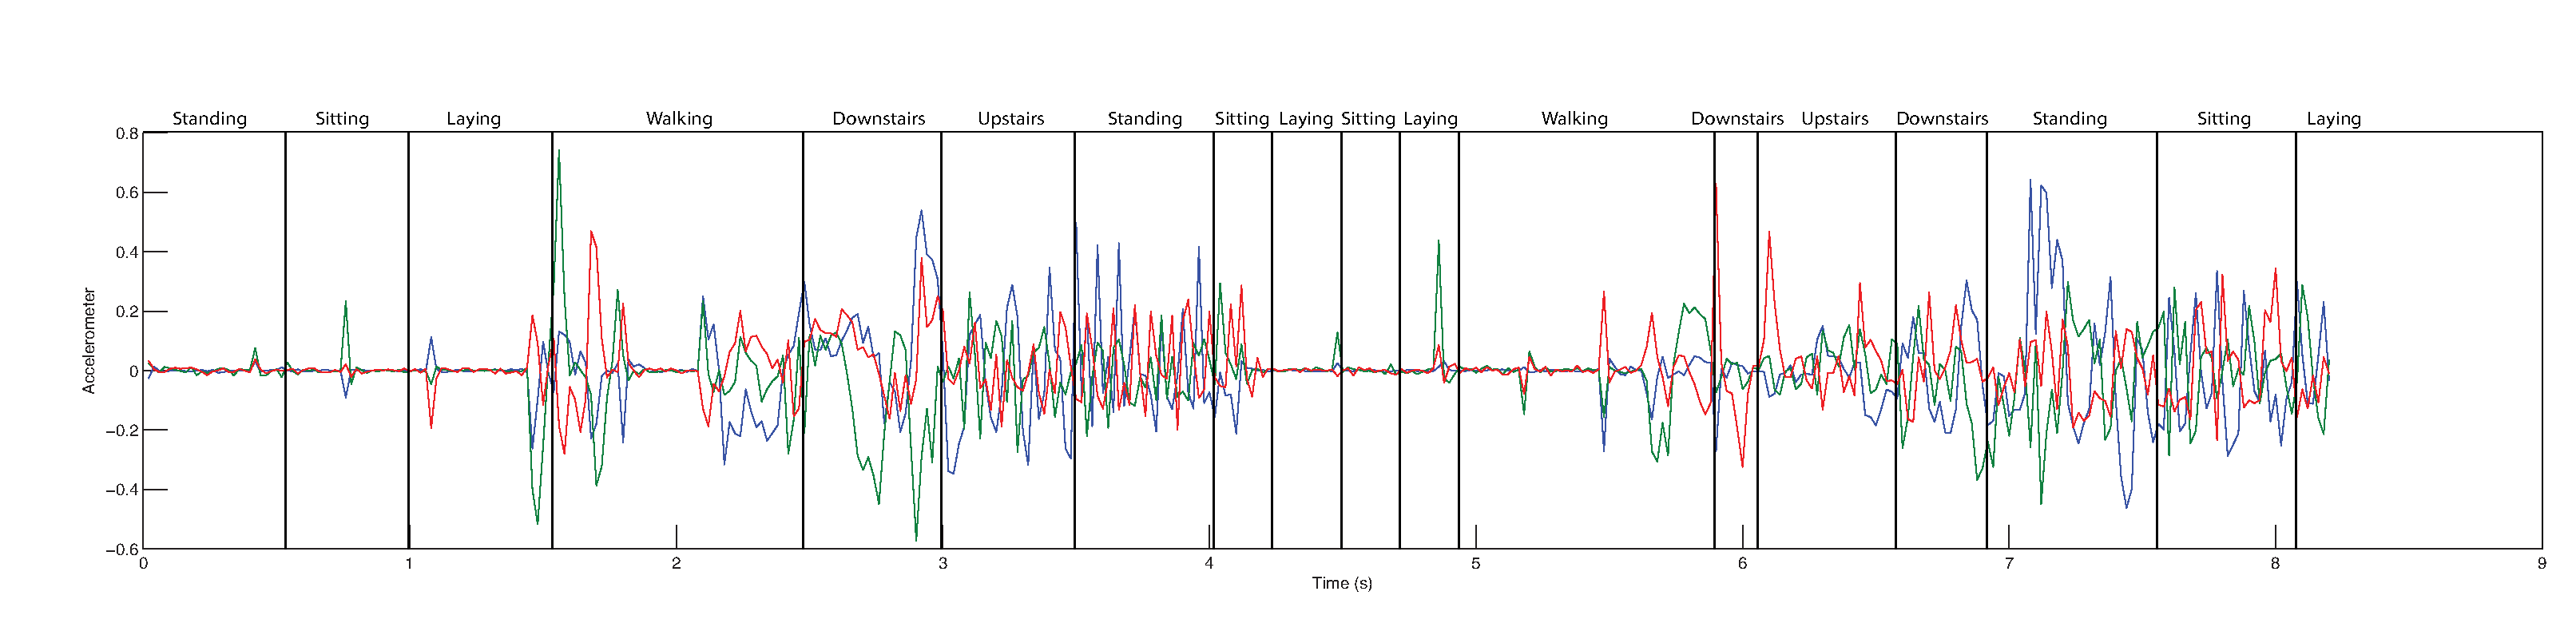
\includegraphics[width=1\textwidth]{./Figures/Chapter6/data_collection/uci_annotated.eps}
  \caption[UCI HAR Excerpt]{Excerpt from the UCI HAR data set \cite{anguita2012human}. The recorded training activities for subject $25$ are displayed. Due to the imprecise (and possibly incorrect) labeling and the short duration of activities, the data set can not be used for the change detection method as described in this thesis.}
  \label{fig:uci_annotated}
\end{figure}

Because of the above described shortcomings of commonly used data sets, we have decided to record activities by ourselves.
The following characterizing requirements were set for our data sets:
\begin{enumerate}
  \item The activities need to be performed and recorded in a continuous manner,
  \item The environment should be natural and uncontrolled, both in- and outdoor,
  \item The data should be clearly annotated, as objective as possible,
  \item The required hardware (and software) should be widely available.
\end{enumerate}

With these requirements in mind, we have created the following setup.
All activities were recorded by a smartphone worn on body in the right front pants pocket of the subject.
The used phones are the \textsc{HTC Sensation XE} and \textsc{HTC Desire}, running the \textsc{Android} smartphone operating system.
During the activities the inertial sensor data is recorded using a free application, \textsc{Sensor Logger}.
This application records the sensor data to \textsc{CSV} files, which are then transformed to \textsc{MATLAB} compatible files.
The constructed algorithm processes the data in an online manner (using only current and historic data).
The \textsc{MATLAB} implementation uses the \gls{svdd} library \textsc{dd\_tools} by Tax \cite{Ddtools2013}.
During the activities, the subject is recorded with a video camera to enable manual labeling and determination of the change points.
As illustrated in the top row of \Cref{fig:stills_subject_1_and_2}, the manual labeling is an ambiguous task.
In \Cref{fig:stills_subject_2_change_point} a transition between walking and running is shown.
It is impossible to determine the exact location of the change point and thus objective quality measures (such as the delay) are of less importance.

Using the video recordings, the data sets are manually annotated, as shown in the plots of \Cref{fig:plots_subject_1,fig:plots_subject_2,fig:plots_subject_3}.
The graphs display each from a single recording the inertial sensor values (see \Cref{tab:recorded_metrics} for explanation of the metrics), with manually annotated activities above the data.
The manually determined change points are used to draw quality conclusion over the algorithm's performance, by comparing it to the discovered change points.
All of the used data sets, including the video material and manual labeling, are made available to the public as the \acrlong{almende-data} \cite{vlasveld2014acras} for further research.
The following section discusses the performed activities during the recordings.
